\section{Não Supervisionado} 

\begin{frame}
    \frametitle{Aprendizado Não Supervisionado}
    \begin{figure}
        \centering
        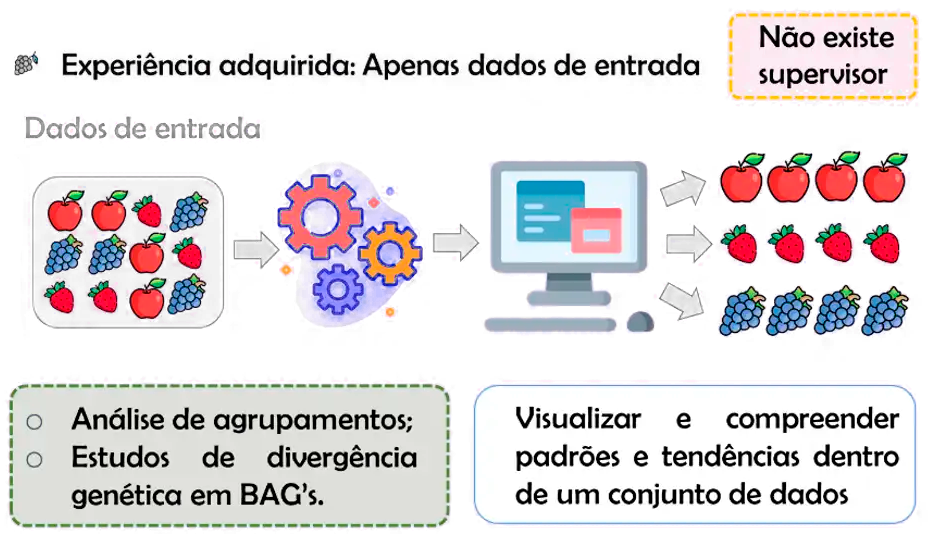
\includegraphics[width=1\linewidth]{img/nao-supervisionado.png}
    \end{figure}
\end{frame}

\begin{frame}
    \frametitle{Agrupamento}
    \begin{itemize}
        \item Identificar e agrupar dados semelhantes com base em características.
        \item O modelo organiza os dados em grupos (clusters) sem rótulos predefinidos.
    \end{itemize}

    \begin{figure}
        \centering
        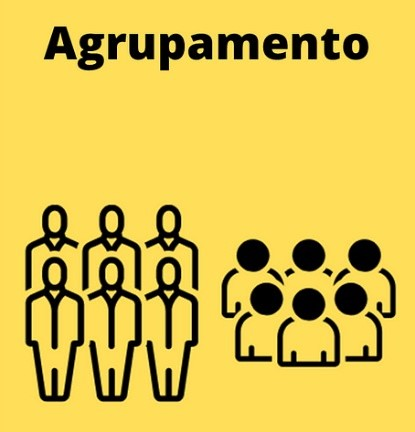
\includegraphics[width=0.3\linewidth]{img/agrupamento.jpg}
        \hspace{0.3cm}
        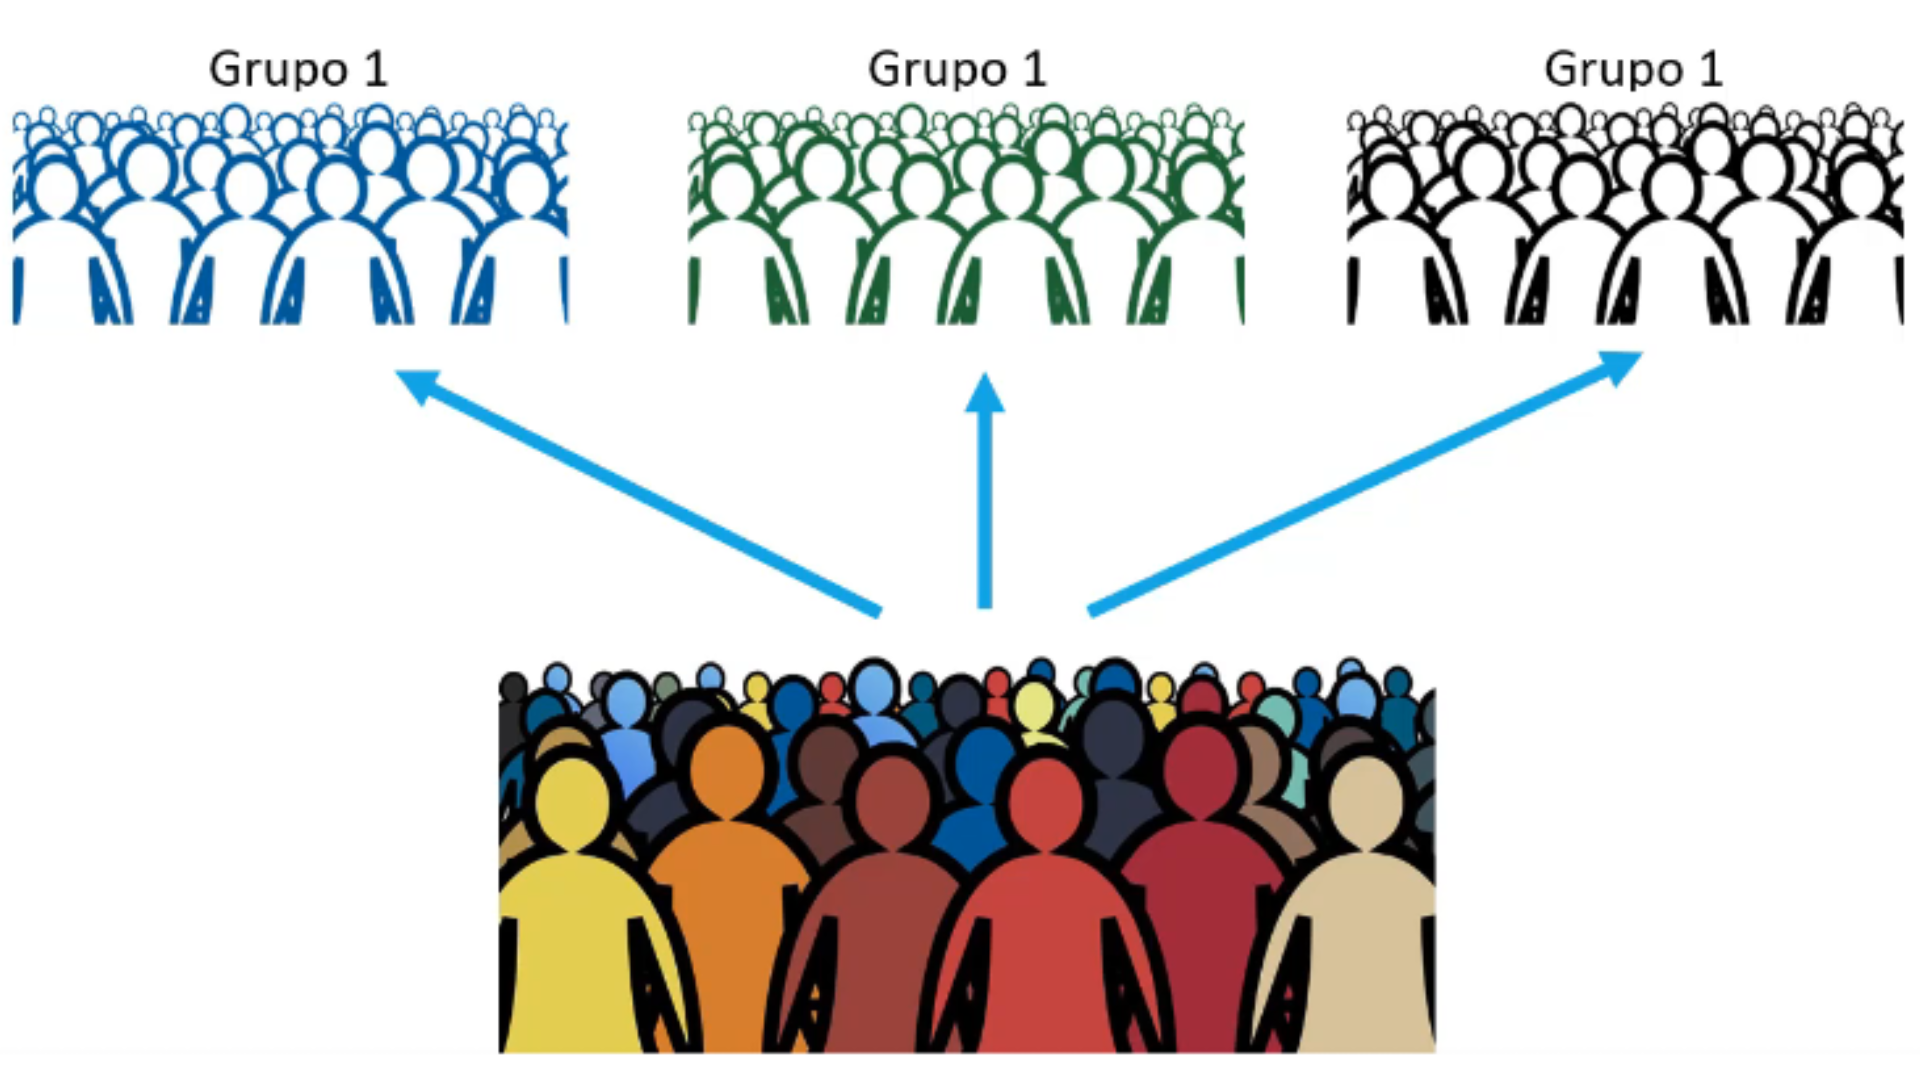
\includegraphics[width=0.6\linewidth]{img/agrupamento.png}
    \end{figure}
\end{frame}

\begin{frame}
    \frametitle{Agrupamento}
    \textbf{Exemplos:}
    \begin{itemize}
        \item \textbf{Segmentação de Clientes:} Agrupar clientes com comportamentos similares para personalização de campanhas (ex.: consumidores frequentes e esporádicos).
        
        \item \textbf{Agrupamento de Imagens:} Organizar imagens com base em semelhanças visuais (ex.: agrupar fotos de paisagens, animais ou objetos).

        \item \textbf{Agrupamento de Dados Geoespaciais:} Agrupar cidades, bairros e regiões com base em características socioeconômicas (renda, mobilidade, infraestrutura) ou ambientais (tipo de solo, cobertura florestal, disponibilidade de água)
    \end{itemize}
\end{frame}

\begin{frame}
    \frametitle{Algoritmos K-Means}
    \begin{itemize}
        \item "K" = Número de centroides (clusters) definidos previamente
        \item  “Means” = Média dos pontos em cada cluster. Determina a posição de seu centroide.
    \end{itemize}
    .
    \begin{figure}
        \centering
        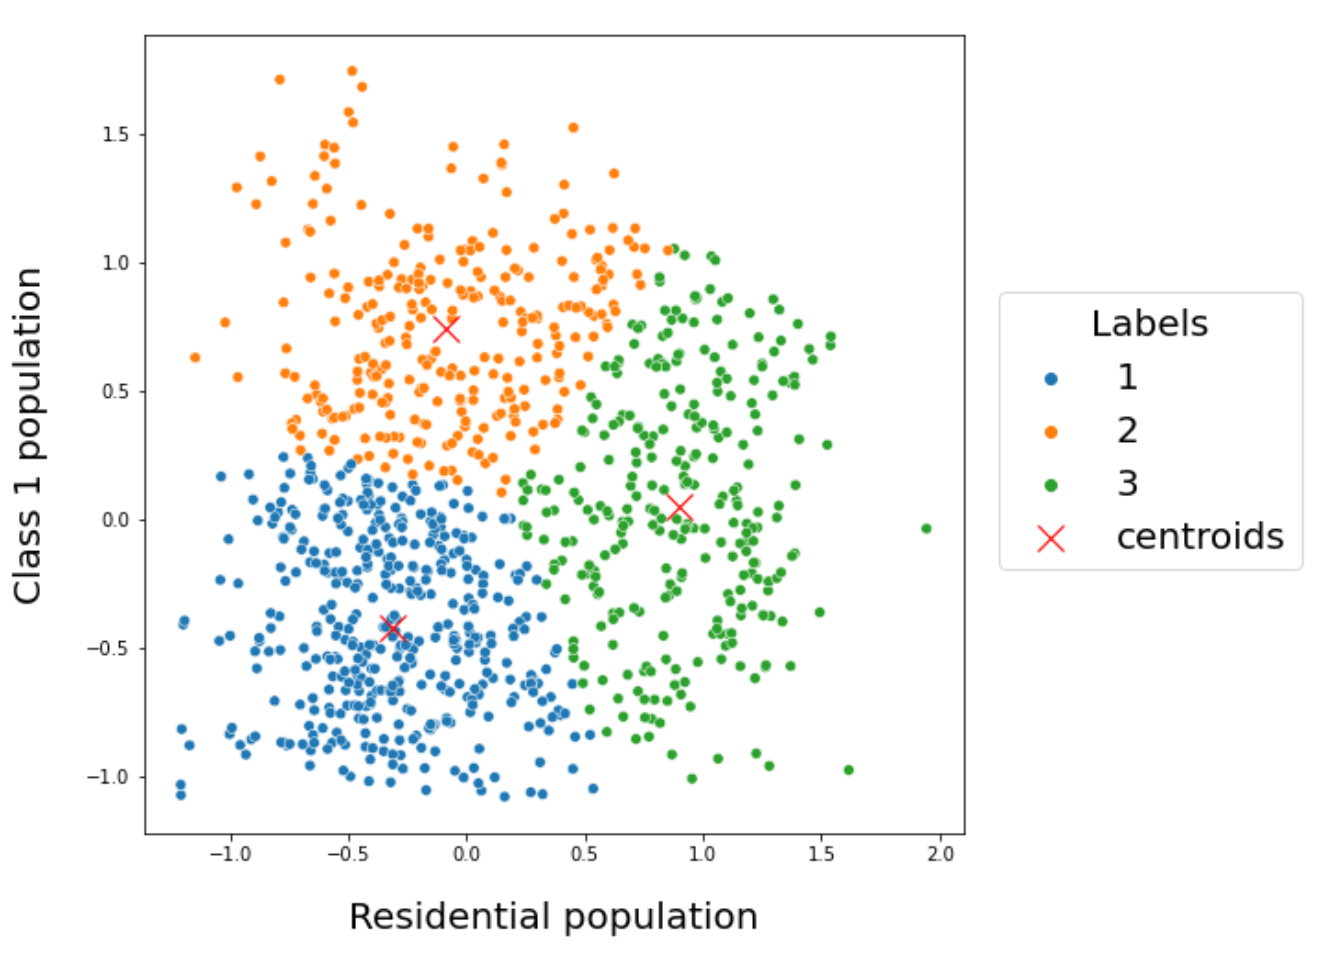
\includegraphics[width=0.5\linewidth]{img/imagekmeans.png}
    \end{figure}
\end{frame}

\begin{frame}
    \frametitle{Algoritmos K-Means}
    \begin{itemize}
        \item Os centroides são posicionado na média dos pontos pertencentes ao seu cluster.
        \item O algoritmo encontra o centroide mais próximo a um novo ponto.
        \item O ponto é então classificado como \textbf{pertencente ao cluster} daquele centroide.
    \end{itemize}
    \begin{figure}
        \centering
        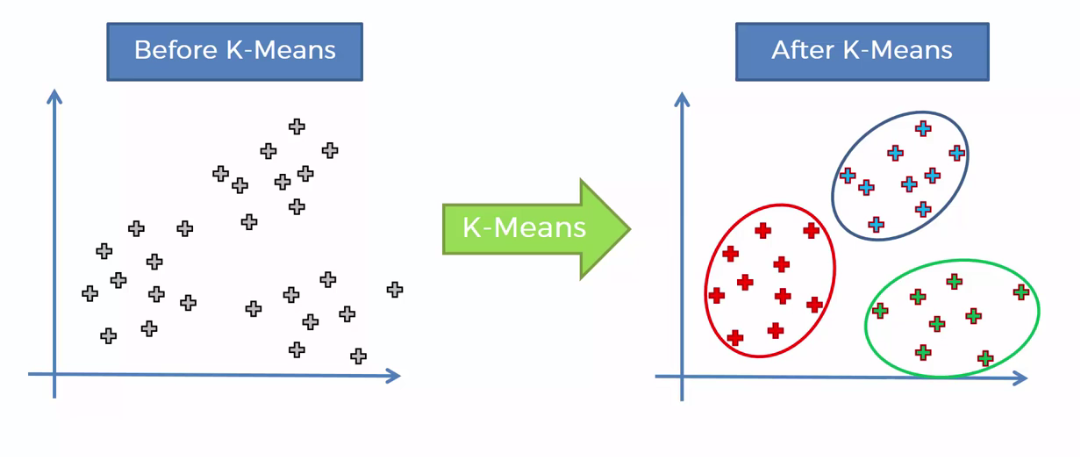
\includegraphics[width=0.5\linewidth]{img/kmeans.png}
    \end{figure}
\end{frame}

\begin{frame}
    \frametitle{Métricas de Avaliação do Agrupamento}
    \textbf{Inércia (Coesão):}
    \begin{itemize}
        \item Mede \textbf{o quão próximos os pontos estão} dentro de um mesmo cluster.
        \item Menores valores =  maior densidade.
        \item Menor distância entre os pontos dentro de um cluster = \textbf{maior a inércia} e mais \textbf{similares} são entre si.
    \end{itemize}

    \textbf{Separação:}
    \begin{itemize}
        \item Avalia a \textbf{distãncia} entre clusters.
        \item Valores maiores = os clusters estão bem separados.
        \item Um \textbf{bom} agrupamento deve ter \textbf{uma alta separação}, significando que os clusters não estão se sobrepondo e são bem distintos entre si.
    \end{itemize}
\end{frame}

\begin{frame}
    \frametitle{Coeficiente de Silhueta (Silhouette Score)}
    \begin{itemize}
        \item Combina a inércia e a separação para fornecer uma \textbf{visão balanceada} da clusterização;
        \item O valor dessa métrica varia de -1 a 1, \item Valor negativo indica que o ponto pode ter sido atribuído ao cluster errado.
    \end{itemize}
    
     \begin{center}
    \[
    Silhueta_{\,\textit{ponto i}} = \frac{\textit{Inercia}_{i} - \textit{Separação}_{i}}{max(\textit{Inércia}_{i}, \textit{Separação}_{i})}
    \]
    \end{center}

\end{frame}

\begin{frame}
    \frametitle{Método do Cotovelo}
    \begin{itemize}
        \item Determina o número ideal de clusters identificando o ponto onde a redução na inércia se torna marginal.
    \end{itemize}

    \begin{figure}
        \centering
        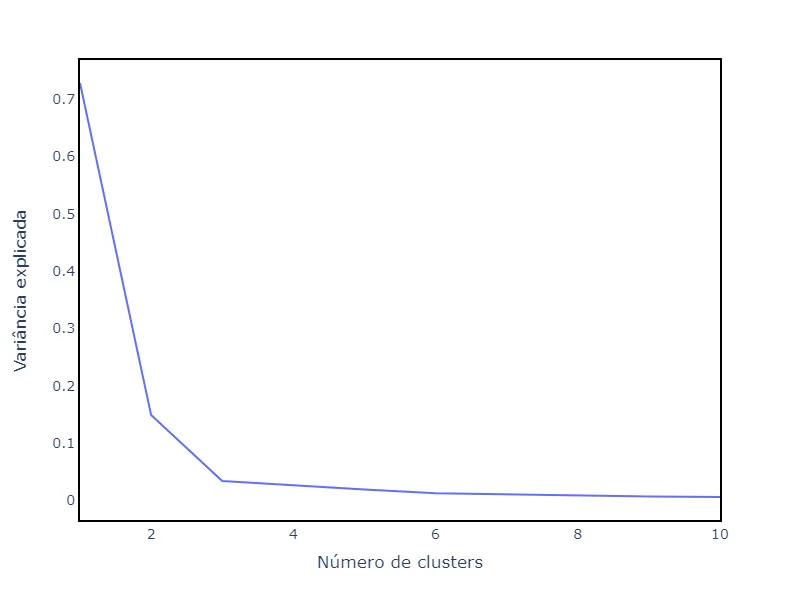
\includegraphics[width=0.6\linewidth]{img/imagecotovelo.png}
    \end{figure}
\end{frame}